\section{Types of Graphs}

A typical graph probably does not have any special characteristics that set that graph apart from others.
There are, however, a whole slew of graphs that are recognized separately from a typical graph.
Among these are complete graphs and bipartite graphs, which we will examine here.

\subsection*{Complete Graphs}

To grasp the concept of a complete graph, we must first understand the idea of connectedness.
We will, as is common in graph theory, begin with a definition.

\begin{definition}{Connected}
	A graph $G$ is called connected if for every pair of vertices $u,v\in V(G)$, there is a $uv$ walk in $G$.
	$G$ is called disconnected if it is not connected.
\end{definition}

In other words, we can get from any vertex to any other vertex in the graph no matter what.
It is especially important to realize that pictures can deceive us here, as the next example will show.

\begin{example}{Determine if the following graph is connected}
	\begin{center}
		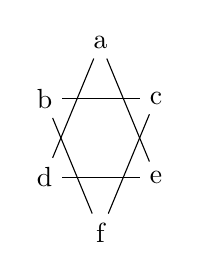
\begin{tikzpicture}[node distance=1cm]
			\node(a) {a};
			\node(b) [below left of=a] {b};
			\node(c) [below right of=a] {c};
			\node(d) [below of=b] {d};
			\node(e) [below of=c] {e};
			\node(f) [below right of=d] {f};

			\draw(a) -- (d);
			\draw(d) -- (e);
			\draw(e) -- (a);
			\draw(b) -- (f);
			\draw(f) -- (c);
			\draw(b) -- (c);
		\end{tikzpicture}
	\end{center}

	As it turns out, this graph is not connected, since there is no $ab$ path, even though the two cycles are drawn on top of each other.
\end{example}

In the above example, we can see two cycles, $adea$ and $bcfb$.
These two cycles are completely disjoint from each other; we cannot start on one and get to the other.
Hence, the two cycles actually form smaller graphs themselves. We call them \textit{subgraphs}

\begin{definition}{Subgraph}
	Suppose $G$ is a graph, and let $H$ be a graph such that $V(H)\subset V(G)$ and $E(H)\subset E(G)$.
	Then $H$ is a subgraph of $G$, denoted by $H\leq G$.
\end{definition}

In our case, we actually have two disconnected subgraphs who together from $G$.
If this is the case, we can take the concept of subgraphs a step further.

\begin{definition}{Connected Component}
	Suppose $G$ is a graph, and let $H$ be a graph such that $H\leq G$. Then $H$ is called a connected component if
	\begin{enumerate}
		\item $H$ is connected
		\item $v\in V(H)$ and $u\in V(G)\setminus V(H) \implies$ there is no $uv$ path in $G$.
	\end{enumerate}
\end{definition}

This is exciting, since we can now say $adea$ and $bcfb$ form connected components of $G$.
Not all graphs will contain connected components, however; if this is the case, we might be interested in trying to create connected components by removing either a vertex or an edge from the graph.
If we can accomplish this, then we call the removed vertices or edges by special names.

\begin{definition}{Cut Vertex}
	Let $G$ be a graph with $v\in V(G)$. Then $v$ is called a cut vertex of $G$ if the graph formed by removing $v$, $G-v$, has more connected components that $G$.
\end{definition}

We need to be a little cautious when we say \textit{remove $v$}; removing a vertex requires us to remove all the edges incident with that vertex as well.

\begin{example}{Determine the cut vertices of the following graph.}
	\begin{center}
		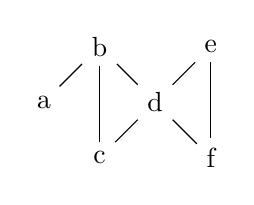
\begin{tikzpicture}[node distance=1cm]
			\node(a) {a};
			\node(b) [above right of=a] {b};
			\node(c) [below right of=a] {c};
			\node(d) [above right of=c] {d};
			\node(e) [above right of=d] {e};
			\node(f) [below right of=d] {f};

			\draw(a) -- (b);
			\draw(b) -- (c);
			\draw(b) -- (d);
			\draw(c) -- (d);
			\draw(d) -- (e);
			\draw(d) -- (f);
			\draw(e) -- (f);
		\end{tikzpicture}
	\end{center}

	We need to identify vertices that create connected components upon their removal. The vertex $d$ does the job here, since $G-d$ looks like

	\begin{center}
		\begin{tikzpicture}[node distance=1cm]
			\node(a) {a};
			\node(b) [above right of=a] {b};
			\node(c) [below right of=a] {c};
			\node(d) [above right of=c] {};
			\node(e) [above right of=d] {e};
			\node(f) [below right of=d] {f};

			\draw(a) -- (b);
			\draw(b) -- (c);
			\draw(e) -- (f);
		\end{tikzpicture}
	\end{center}
	where one connected component is given by the vertices $abc$ and the other by the vertices $ef$.
	There is another vertex that works here: $b$. Note that a single vertex is connected by definition, and $G-b$ looks like
	\begin{center}
		\begin{tikzpicture}[node distance=1cm]
			\node(a) {a};
			\node(b) [above right of=a] {};
			\node(c) [below right of=a] {c};
			\node(d) [above right of=c] {d};
			\node(e) [above right of=d] {e};
			\node(f) [below right of=d] {f};

			\draw(c) -- (d);
			\draw(d) -- (e);
			\draw(d) -- (f);
			\draw(e) -- (f);
		\end{tikzpicture}
	\end{center}

	where $a$ is one connected component and $c,d,e,$ and $f$ are in the other connected component.
\end{example}

Similarly, we have a definition for edges that accomplish this task.
Removal of edges is simpler than vertices, however, since we need not worry about the vertices incident with the edge.

\begin{definition}{Bridge}
	Let $G$ be a graph with $e\in E(G)$. Then $e$ is called a bridge of $G$ if the graph formed by removing $e$, $G-e$, contains more connected components than $G$.
\end{definition}

Vertices seem to be the more interesting object to remove from a graph, so we will focus on them a little more than edges.
We have a special name for the set of vertices that are cut verticies.

\begin{definition}{Cut Set}
	Let $G$ be a graph and let $S\subset V(G)$. $S$ is called a cut set of $G$ if the graph with vertex set $V(G)\setminus S$ is disconnected.
\end{definition}

In other words, if we remove all the cut vertices from a graph, we expect that graph to be disconnected.
Indeed, this makes intuitive sense, since any graph with more than one connected component is disconnected, and cut vertices create connected components.
With the notion of cut set, we can finally introduce completeness of graphs.

\begin{definition}{Complete}
	Let $G$ be a graph. $G$ is called complete if and only if $G$ has no cut sets.
	We denote a complete graph by $K_{n}$ where $n=ord(G)$.
\end{definition}

A complete graph consists of $n$ vertices that have every edge possible; hence removing one of the vertices isn't a problem since every other vertex is still connected to any other vertex in the graph.

\begin{example}{}
	The following are examples of complete graphs.
	\begin{center}
		\begin{tabular}{c c c}
			\begin{tikzpicture}[node distance=1cm]
                \node(a) {a};
                \node(b) [left of=a] {b};

                \draw(a) -- (b);
			\end{tikzpicture} &
			\begin{tikzpicture}[node distance=1cm]
                \node(a) {a};
                \node(b) [below right of=a] {b};
                \node(c) [above right of=b] {c};

                \draw(a) -- (b);
                \draw(b) -- (c);
                \draw(c) -- (a);
			\end{tikzpicture} &
			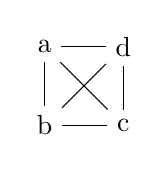
\begin{tikzpicture}[node distance=1cm]
                \node(a) {a};
                \node(b) [below of=a] {b};
                \node(c) [right of=b] {c};
                \node(d) [above of=c] {d};

                \draw(a) -- (b);
                \draw(a) -- (c);
                \draw(a) -- (d);
                \draw(b) -- (c);
                \draw(b) -- (d);
                \draw(c) -- (d);
			\end{tikzpicture}\\
            $K_{2}$ & $K_{3}$ & $K_{4}$
		\end{tabular}
	\end{center}
\end{example}

\subsection*{Bipartite Graphs}

The next type of graph we will study is called a bipartite graph.
Bipartite graphs are unique in that they can be partitioned into two sets that contain disconnected vertices.

\begin{definition}{Bipartite}
    Let $G$ be a graph and let $W\subset V(G)$. $G$ is called bipartite if for every edge in $uv\in E(G)$, either $u\in W$ and $v\in V(G)\setminus W$, or $u\in V(G)\setminus W$ and $v\in W$.
\end{definition}
